%===================================================================================
% FESTIVAL DE LA CLASE - MATCOM, UH
%===================================================================================
% Esta plantilla ha sido diseñada para ser usada en los artículos del Festival de 
% la Clase de MatCom.
%
% Por favor, siga las instrucciones de esta plantilla y rellene en las secciones
% correspondientes.
%
% NOTA: Necesitará el archivo 'fc_jcematcom.sty' en la misma carpeta donde esté este
%       archivo para poder utilizar esta plantila.
%===================================================================================



%===================================================================================
% PREÁMBULO
%-----------------------------------------------------------------------------------
\documentclass[a4paper,10pt,twocolumn]{article}

%===================================================================================
% Paquetes
%-----------------------------------------------------------------------------------
\usepackage{amsmath}
\usepackage{amsfonts}
\usepackage{amssymb}
\usepackage{amsthm}
\usepackage{fc_jcematcom}
\usepackage[utf8]{inputenc}
\usepackage{listings}
\usepackage[pdftex]{hyperref}
\usepackage{caption}
\usepackage{subcaption}
%-----------------------------------------------------------------------------------
% Configuración
%-----------------------------------------------------------------------------------
\hypersetup{colorlinks,%
	    citecolor=black,%
	    filecolor=black,%
	    linkcolor=black,%
	    urlcolor=blue}
%-----------------------------------------------------------------------------------
% Teoremas y definiciones
%-----------------------------------------------------------------------------------
\theoremstyle{theorem}
\newtheorem{thm}{Teorema}[section]
\theoremstyle{definition}
\newtheorem{cor}[thm]{Corolario}
\newtheorem{lem}[thm]{Lema}
\newtheorem{prop}[thm]{Proposición}
\newtheorem{defn}[thm]{Definición}
\newtheorem{ejem}[thm]{Ejemplo}
\newtheorem{ejer}[thm]{Ejercicio}
\theoremstyle{remark}
\newtheorem{obs}[thm]{Observación}
%===================================================================================



%===================================================================================
% Presentacion
%-----------------------------------------------------------------------------------
% Título
%-----------------------------------------------------------------------------------
\title{Modelación de Problemas Lineales de Optimización\\
\vspace{2ex}
\begin{large}
Modelos de Optimización\\
Lic. en Ciencias de la Computación
\end{large}}

%-----------------------------------------------------------------------------------
% Autores
%-----------------------------------------------------------------------------------
\author{\\
\name Luis Ernesto Ibarra Vázquez \email \href{mailto:luis.ibarra@estudiantes.matcom.uh.cu}{luis.ibarra@estudiantes.matcom.uh.cu}
	\\ \addr Grupo C411 \\
\name Adrián Hernández Pérez \email \href{mailto:adrianmatcom@gmail.com}{adrianmatcom@gmail.com}
	\\ \addr Grupo C411 \\
\name Damián O'Hallorans Toledo \email \href{mailto:luis.ibarra@estudiantes.matcom.uh.cu}{luis.ibarra@estudiantes.matcom.uh.cu}
	\\ \addr Grupo C412} % TODO Correo

%-----------------------------------------------------------------------------------
% Tutores
%-----------------------------------------------------------------------------------
\tutors{\\
MsC. Fernando Rodríquez, \emph{Universidad de La Habana}}

%-----------------------------------------------------------------------------------
% Headings
%-----------------------------------------------------------------------------------
\jcematcomheading{\the\year}{1-\pageref{end}}{Luis Ernesto Ibarra, Adrián Hernández, Damián O'Hallorans}

%-----------------------------------------------------------------------------------
\ShortHeadings{Clase Práctica: Modelación de Problemas Lineales}{Luis Ernesto Ibarra, Adrián Hernández, Damián O'Hallorans}
%===================================================================================



%===================================================================================
% DOCUMENTO
%-----------------------------------------------------------------------------------
\begin{document}

%-----------------------------------------------------------------------------------
% NO BORRAR ESTA LINEA!
%-----------------------------------------------------------------------------------
\twocolumn[
%-----------------------------------------------------------------------------------

\maketitle

%===================================================================================
% Lenguaje
%-----------------------------------------------------------------------------------
\selectlanguage{spanish} % Para producir el documento en Español
\vspace{0.5cm}
]

%===================================================================================
% Objetivos
%-----------------------------------------------------------------------------------
\section{Objetivos}
%-----------------------------------------------------------------------------------
\begin{enumerate}
	\item Recordar las definciones básicas sobre la asignatura dadas en conferencia
	\item Modelar tipos de problemas comunes en la optimización lineal
%	\item Esta sección va dedicada a los objetivos de la clase, las metas para el encuentro y ciertas especificidades que considere de importancia resaltar durante el trancurso de la clase.
%	\item Según la temática se puede hacer alusión a los medios de enseñanza utilizados.
\end{enumerate}


%===================================================================================
% Introducción
%-----------------------------------------------------------------------------------
\section{Introducción}\label{sec:intro}
%-----------------------------------------------------------------------------------
(Este segmento tiene una duración de $5$ minutos.)\\

Se introduce la clase que se ambienta en el popular mundo de Juego de Tronos como medio para motivar a los estudiantes en la realización de los ejercicios. En concreto se creó con la idea de la preparación para la batalla conocida como The Long Night, bastante famosa en la serie. En los ejericios se tienen que reunir, crear y transportar recursos eficientemente para luego poder sobrevivir al combate contra los caminantes blancos. Los ejercicios abarcan un abanico de problemas diferentes que se ven comúnmente en la optimización lineal.\\

Se dividirá el aula en dos equipos para fomentar la competitividad durante el transcurso de la clase, los equipos se llamarán en dependencia de las regiones en que se divide el continente:

\begin{itemize}

	\item Riverlands
	\item Vale of Arryn

\end{itemize}

Se explicará el flujo de la clase, el cual consiste en:

\begin{enumerate}

	\item Plantear el modelo que resuelve el ejercicio.
	\item Pedir a cada equipo los diferentes valores de las variables de decisión.
	\item El equipo que más se acerque al resultado óptimo obtendrá un punto.
	\item El equipo que más puntos tenga al final, gana.

\end{enumerate}

%===================================================================================
% Desarrollo
%-----------------------------------------------------------------------------------
\section{Teorizando un poco}\label{sec:teoria}
%-----------------------------------------------------------------------------------
(Este segmento tiene una duración de $10$ minutos)\\

En la conferencia previa a la clase práctica se deben de haber dado los temas introductorios con la optimización general y también algunos problemas clásicos de la optimización lineal. En un principio se tocará brevemente estos puntos para recordar las definiciones y construcciones.

Se plantearán las siguientes preguntas a los estudiantes:

%-----------------------------------------------------------------------------------
	\subsection{¿Qué es un modelo matemático?}\label{sub:results}
%-----------------------------------------------------------------------------------

Esta pregunta se realizará con el objetivo de introducir la representación de problemas del mundo real al mundo matemático y su representación computacional.\\

Un modelo matemático es una abstracción de un problema real, formulado matemáticamente, que tiene como objetivo reproducir el problema en cuestión de la forma más fiel posible con el fin de poder entender y estudiar cómo se comporta.\\

Un ejemplo problema sencillo de modelación que se podría presentar sería cómo modelar una imagen. En este caso el modelo matemático que se usaría serían las matrices. Con estas se puede representar una imagen asignando cada color en la imagen real a un número en la matriz en la posición correspondiente. 

%-----------------------------------------------------------------------------------
	\subsection{¿Qué es un modelo de optimización?}\label{sub:results}
%-----------------------------------------------------------------------------------

Esta pregunta se realizará con el objetivo de especificar el tipo de problemas que se trata en la asignatura y llegar al Problema General de Optimización Matemática (PGOM).\\

Un modelo de optimización es uno en donde se quiere hallar el mínimo o máximo de cierta función. Se define como Problema General de Optimizazción Matemática al problema P siguiente:

$$
P: \min f(x)
$$
$$
s.a. \quad h_i(x) = 0 \quad i \in \{1,...,m\}
$$
$$
\qquad \qquad \qquad g_j(x) \le 0 \quad j \in \{m+1,...,m+k\}
$$
$$
\quad x \in \Omega
$$

%-----------------------------------------------------------------------------------
		\subsubsection{Ejemplo}\label{subsub:ejemplo}
%-----------------------------------------------------------------------------------

Se muestra un ejemplo concreto sencillo que luego servirá de referencia para las futuras preguntas, presentando preguntas escenciales a la hora de modelar:\\

Tyrion Lannister se está quedando sin bebidas alcohólicas, entonces haciendo alusión a su célebre frase, \textit{“Eso se lo que hago, bebo y sé cosas”} quiere hacer su propia bebida. Para esto cuenta con 30 libras de uvas, 40 libras de cebada y con 30 libras de levadura. Él conoce que para crear un litro de cerveza necesita 1 libra de cebada y 0.5 libras de levadura, mientras que para crear vino los requisitos son 2 libras de uva y 1 libra de levadura. Conociendo que la cerveza tiene un nivel de alcohol de 2\% y el vino 4\%, ¿cuál es la mejor manera de distribuir los recursos para crear la mayor cantidad de alcohol?\\

\textbf{¿Qué hay que decidir?}

\begin{itemize}
	\item $c$: Cantidad de litros de cerveza producido.
	\item $v$: Cantidad de litros de vino producido.
\end{itemize}

\textbf{¿Qué se quiere maximizar o minimizar?}

$$
P: \max f(c, v) = c * 0.02 + v * 0.04
$$

\textbf{¿Cuáles son las condiciones que tiene que cumplir el problema?}

$$
s.a. \quad 2 v \le 30
$$
$$
\qquad c \le 40
$$
$$
\qquad \qquad 0.5 c + v \le 30 
$$
$$
\qquad 0 \le c 
$$
$$
\qquad 0 \le v 
$$
$$
\quad x = (c, v) \in R^2
$$

%-----------------------------------------------------------------------------------
	\subsection{¿Cuáles son las partes de un PGOM?}\label{sub:results}
%-----------------------------------------------------------------------------------

Esta pregunta se realizará con el objetivo de mencionar y explicar las diferentes partes que componen a un PGOM y la función que realiza cada una de ellas.

%-----------------------------------------------------------------------------------
		\subsubsection{Partes de un PGOM}\label{subsub:partes}
%-----------------------------------------------------------------------------------

\textbf{Variables de decisión:} Se asocian a las decisiones que se pueden tomar en el problema. Ejemplo, cantidad de productos a producir de cada tipo. Ejemplo $c,v$. Ver \ref{subsub:ejemplo}.  

\textbf{Función objetivo:} Es la función que se desea encotrar el óptimo, expresa el objetivo del problema. Ejemplo: $f(c, v)$. Ver \ref{subsub:ejemplo}.

\textbf{Restricciones:} Conjunto de restricciones que tienen que cumplir las variables de decisión para que el problema tenga solución. Ejemplo: $ 2 v \le 30$, $c \le 40$, $0.5 c + v \le 30 $, $0 \le c$ y $0 \le v$. Ver \ref{subsub:ejemplo}.

%-----------------------------------------------------------------------------------
	\subsection{¿Qué significa resolver un PGOM?}\label{sub:results}
%-----------------------------------------------------------------------------------

Esta pregunta se realizará con el objetivo de recordar conceptos relacionados con el conjunto solución, dígase soluciones factibles y soluciones óptimas.

%-----------------------------------------------------------------------------------
		\subsubsection{Conjuntos y Soluciones}\label{subsub:solucion}
%-----------------------------------------------------------------------------------

\textbf{Conjunto de soluciones factibles ($M \subset \Omega$):} Conjunto de valores que toman las variables de decisión que satisfacen las restricciones del problema. Ejemplo: $x = (c, v) = (0, 0)$ o $x = (c, v) = (1, 2)$. Ver \ref{subsub:ejemplo}.

\textbf{Solución óptima ($x^*$):} Mínimo o máximo global de la función objetivo sobre $M$. Ejemplo: $x^* = (c, v) = (30, 15)$. Ver \ref{subsub:ejemplo}.

%===================================================================================
% Ejercicios resueltos
%-----------------------------------------------------------------------------------
\section{Ejercicios}\label{sec:ejer}
%-----------------------------------------------------------------------------------
Se realiza una introducción a los ejercicios basada en la historia de la serie y en el contexto en que se encuentran, en la preparación de la la batalla contra los caminantes blancos.\\

Los ejercicios se dividen por algunas de las diferente Casas que participaron en la batalla, para usar la temática de la clase práctica a nuestro favor y darle un mejor ambiente.\\

Una vez esté resuelto el modelo de cada ejercicio, se le pedirá a un integrante de cada equipo que le asigne valores a las variables de acuerdo a su criterio. El resultado se verificará con el programa escrito para la clase, el cual ayuda en la tarea de indicar qué tan bueno es su resulado. Finalmente se le da el punto al equipo que más se acerque al óptimo.

%-----------------------------------------------------------------------------------
	\subsection{Casa Mormont}\label{subsec:ejer_1}
%-----------------------------------------------------------------------------------
(Este ejercicio tiene una duración de $10$ minutos.)\\

En la preparación de la batalla se necesitan armas para que los guerreros puedan defenderse del ejército de caminantes blancos. Para esto se tienen escasos recursos, así que hay que usarlos sabiamente. Entre las reservas y el trabajo se logró reunir:

\begin{itemize}

	\item 300 unidades de hierro
	\item 400 unidades de madera
	\item 400 unidades de cuero

\end{itemize}

Los herreros y artesanos nos brindan una tabla que muestra la cantidad de materia prima necesaria para construir cada arma y el daño que reporta cada una.

\begin{figure}[h!]%
	\begin{center}
		\begin{tabular}{|c|c|c|c|c|} \hline
		Arma		& Hierro 	& Madera 	& Cuero   & Daño    \\ \hline
		Espada		& 10		&  2		&  4	  & 15		\\ \hline
		Arco		&  2		& 10		&  5	  & 10		\\ \hline
		Catapulta	& 30		&100		& 50	  & 80		\\ \hline
		\end{tabular}
	\caption{Datos de armas}\label{fig:ejer_1}
	\end{center}
\end{figure}

\renewcommand{\theenumi}{\alph{enumi}} % enumerate con incisos
% \renewcommand{\theenumi}{\arabic{enumi}} % enumerate con números

\begin{enumerate}

	\item Ayude a darle el mejor uso a estos recursos, diciéndoles a los jefes de la casa la cantidad de espadas, arcos y catapultas que 
	necesitan construir para maximizar el daño que realizan.
	\item Se quiere tener modelo que generalice el problema anterior en términos de la cantidad de tipos de materiales y cantidad de tipos de 
	armas. Proponga un modelo que haga esta generalización.

\end{enumerate}

%-----------------------------------------------------------------------------------
		\subsubsection{Sobre el ejercicio}\label{subsubsec:sobre_ejer_1}
%-----------------------------------------------------------------------------------

Este ejercicio es un sencillo problema de producción, en el cual se tienen materiales y productos que se construyen con estos materiales y se quiere maximizar la utilidad de los productos, el daño en este caso. Una vez se haga el primer inciso los estudiantes deben de poder generalizar el problema para que el modelo sea independiente de la cantidad de tipos de materiales y productos. Esto último brindará al estudiante de conocimiento práctico sobre el uso de sumatorias, vectores y matrices para trabajar con problemas de optimización, ya que se verán obligados a no solo usar ecuaciones fijas para las restricciones y función objetivo.

%-----------------------------------------------------------------------------------
		\subsubsection{Solución}\label{subsubsec:sol_ejer_1}
%-----------------------------------------------------------------------------------

Inciso a)

\textbf{Variables de decisión:}

\begin{itemize}
	\item $x_1$: Cantidad de espadas.
	\item $x_2$: Cantidad de arcos.
	\item $x_3$: Cantidad de catapultas.		
\end{itemize}

\textbf{Restricciones:}

La cantidad de hierro disponible no puede ser superada:

$$
10x_1 + 2x_2 + 80x_3 \le 300
$$

La cantidad de hierro disponible no puede ser superada:

$$
2x_1 + 10x_2 + 100x_3 \le 400
$$

La cantidad de hierro disponible no puede ser superada:

$$
4x_1 + 5x_2 + 50x_3 \le 400
$$

Las cantidades tienen que ser no negativas:

$$
x_i \ge 0 \quad \forall i \in [1,2,3]
$$

\textbf{Función objetivo:}

Se quiere maximizar el daño inflingido con las armas creadas.

$$
\max 15 * x_1 + 10 * x_2 + 80 * x_3
$$

Inciso b)

\textbf{Variables de decisión:}

\begin{itemize}
	\item $x_i$: Cantidad de producto $i$.
\end{itemize}

\textbf{Restricciones:}

\begin{itemize}
	\item $b_j$: Cantidad de materia prima $j$.
	\item $c_i$: Utilidad del producto $i$.
	\item $a_{ij}$: Cantidad de materia prima $j$ necesitada por producto $i$.
\end{itemize}

Cumpliendo las restricciones de materia prima:

$$
\sum_{i=1} x_i a_{ij} \le b_j \quad \forall j
$$

Las cantidades tienen que ser no negativas:

$$
x_i \ge 0 \quad \forall i
$$

\textbf{Función objetivo:}

$$
\max \sum_{i=1} c_i x_i
$$

%-----------------------------------------------------------------------------------
	\subsection{Casa Greyjoy}\label{subsec:ejer_2}
%-----------------------------------------------------------------------------------
(Este ejercicio tiene una duración de $10$ minutos.)\\

Un importante recurso para la contienda es la comida. Los soldados y la mano de obra son muchos y cada uno necesita ser alimentado para poder trabajar y luchar contra los temibles caminantes blancos. Esta responsabilidad cae sobre Casa Greyjoy. Los cálculos estiman que para hacer una comida para una persona se necesitan:

\begin{itemize}

	\item 60  gramos de proteína
	\item 120 gramos de carbohidratos
	\item 20  gramos de aceite
	\item 1.5 litros de agua

\end{itemize}

Para satisfacer esta demanda se tienen un conjunto de alimentos y ganado a disposición, cada uno aportando diferentes cantidades de nutrientes.

\begin{figure}[h!]%
	\begin{center}
		\begin{tabular}{|c|c|c|c|c|} \hline
		Recurso		& Proteína 	& Carb. 	& Aceite   & Costo  \\ \hline
		Trigo		& 10		& 40				& 20	  & 10		\\ \hline
		Ganado		&100		& 10				& 50	  & 60		\\ \hline
		Encurtido	& 20		& 30				& 10	  & 30		\\ \hline
		Agua		& -			& -					& -		  & 5		\\ \hline
		\end{tabular}
	\caption{Datos de alimentos}\label{fig:ejer_2}
	\end{center}
\end{figure}

\renewcommand{\theenumi}{\alph{enumi}} % enumerate con incisos
% \renewcommand{\theenumi}{\arabic{enumi}} % enumerate con números

\begin{enumerate}

	\item Sabiendo que se espera un ejército de alrededor 10 000 personas, proponga a los jefes de la casa una manera de cumplir con los 
	requerimientos con el menor costo posible.
	\item Se quiere tener modelo que generalice el problema anterior en términos de la cantidad de tipos de nutrientes y cantidad de tipos de 
	recursos. Proponga un modelo que haga esta generalización.

\end{enumerate}

%-----------------------------------------------------------------------------------
		\subsubsection{Sobre el ejercicio}\label{subsubsec:sobre_ejer_2}
%-----------------------------------------------------------------------------------

Este ejercicio es un sencillo problema de dieta, en el cual se tienen alimentos y nutrientes y hace falta suplir las necesidades alimenticias de una persona o grupo de personas gastando la menor cantidad de dinero al comprar alimentos. Al igual que en el primer ejercicio los estudiantes, una vez resuelto el primer inciso, deben de poder generalizar el problema independientemente de la cantidad de tipos de nutrientes y recursos.

%-----------------------------------------------------------------------------------
		\subsubsection{Solución}\label{subsubsec:sol_ejer_2}
%-----------------------------------------------------------------------------------

\textbf{Variables:}

\begin{itemize}

\item $V_{i}$ : El valor de costo del producto $i$.

\item $P_{i}$ : Cantidad de prote\'inas que contiene el producto $i$.

\item $C_{i}$ : Cantidad de carbohidratos que contiene el producto $i$.

\item $A_{i}$ : Cantidad de aceite que contiene el producto $i$.

\item $N_{Y}$ : Cantidad del nutriente $Y$ por persona ($Y$ se\'ria igual a $P$, $C$, $A$ o $Ag$ para prote\'inas, carbohidratos , aceite y agua respectivamente).

\item $T$ : Total de personas.

\end{itemize}

\textbf{Variables de Decisi\'on:}

\begin{itemize}

\item $X_{i}$ : Cantidad a producir del producto $i$.

\end{itemize}

\textbf{Funci\'on objetivo:}

Se desea hallar, cumpliendo los requisitos requeridos para los alimentos de cada persona, el menor costo de producci\'on.

$$
\min \sum^{4}_{i=1} V_{i}X_{i}
$$

\textbf{Restricciones:}

Los requisitos para una comida satisfactoria por persona quedan dados en la descripci\'on del problema, pero quedan descritos de la siguiente forma:

$$
\sum^{4}_{i=1} X_{i} C_{i} \geq N_{C} T
$$

$$
\sum^{4}_{i=1} X_{i} P_{i} \geq N_{P} T
$$

$$
\sum^{4}_{i=1} X_{i} A_{i} \geq N_{A} T
$$

$$
X_{4} \geq N_{Ag} T
$$


%-----------------------------------------------------------------------------------
	\subsection{Casa Targaryen}\label{subsec:ejer_3}
%-----------------------------------------------------------------------------------
(Este ejercicio tiene una duración de $10$ minutos.)\\

El fuego valiryo posee un gran poder ofensivo, este fuego verde arde incluso en el agua y es incapaz de extinguirlo una vez se prende, solo terminando de arder cuando se consume completamente. Las armas imbuidas en este elemento presentan un poder ofensivo superior y además pueden ser usado como bombas incendiarias, así que la producción de este es indispensable. Para fabricar el fuego valiryo se necesita mezclar ciertos ingredientes cuyos nombres no fueron revelados, pero, se conoce la proporción de estos en diferentes recursos naturales:

\begin{figure}[h!]%
	\begin{center}
		\begin{tabular}{|c|c|c|c|c|} \hline
		Recurso				& Ingr. 1 & Ingr. 2 	& Ingr. 3   & Costo  \\ \hline
		Aceite de ballena	& 40\%			& 10\%				& 30\%			  & 40		\\ \hline
		Polvo de dragón		& 10\%			&  5\%				& 50\%	  		  & 70		\\ \hline
		Piel de caballo		& 15\%			& 35\%				&  5\%	  		  & 30		\\ \hline
		\end{tabular}
	\caption{Datos de materiales}\label{fig:ejer_3}
	\end{center}
\end{figure}

Los alquimistas tienen destilados ya:

\begin{itemize}

	\item Ingrediente 1: 15 litros
	\item Ingrediente 2: 30 litros
	\item Ingrediente 3: 10 litros

\end{itemize}

El fuego valiryo está conformado por un 30\% de Ingrediente 1, 20\% de Ingrediente 2 y 50\% de Ingrediente 3. Como dato adicional los alquimistas necesitan procesar el residuo de los recursos para conservar la pureza del fuego, para esto se tiene un costo extra de 5 por cada unidad de material de desecho. Se cuenta como residuo las cantidades que no son ingredientes del fuego que sale del procesamiento de los recursos, por ejemplo el uno de una unidad de aceite de ballena produce 0.2 unidades de residuo.

\renewcommand{\theenumi}{\alph{enumi}} % enumerate con incisos
% \renewcommand{\theenumi}{\arabic{enumi}} % enumerate con números

\begin{enumerate}

	\item Ayude a los alquimistas a crear 100 unidades de fuego valiryo con el menor costo posible para enfrentar al enemigo.

\end{enumerate}

%-----------------------------------------------------------------------------------
		\subsubsection{Sobre el ejercicio}\label{subsubsec:sobre_ejer_3}
%-----------------------------------------------------------------------------------

Este ejercicio es un clásico problema de mezlca en el cual se tienen diferentes materiales con diferentes concentraciones de ingredientes y se quiere crear un producto final con diferentes concentraciones de ingredientes, comprando la menor cantidad de materiales posibles. Al problema base se le agregó una dificultad extra que consiste en eliminar las impurezas de usar los diferentes materiales.

%-----------------------------------------------------------------------------------
		\subsubsection{Solución}\label{subsubsec:sol_ejer_3}
%-----------------------------------------------------------------------------------

\textbf{Variables de decisión:}

\begin{itemize}
	\item $x_1$: Cantidad de aceite de ballena.
	\item $x_2$: Cantidad de polvo de dragón.
	\item $x_3$: Cantidad de piel de caballo.
	\item $x_4$: Cantidad de ingrediente 1.
	\item $x_5$: Cantidad de ingrediente 2.
	\item $x_6$: Cantidad de ingrediente 3.
\end{itemize}

\textbf{Restricciones:}\\

El total de ingrediente 1 representa el 30\%:

$$
0.4 x_1 + 0.1 x_2 + 0.15 x_3 + x_4 = 0.3*100
$$

El total de ingrediente 2 representa el 20\%:

$$
0.1 x_1 + 0.05 x_2 + 0.5 x_3 + x_5 = 0.2*100
$$

El total de ingrediente 3 representa el 50\%:

$$
0.3 x_1 + 0.5 x_2 + 0.05 x_3 + x_6 = 0.5*100
$$

La cantidad de los ingredientes destilados no puede superar la reserva de cada uno:

$$
x_4 \le 15
$$
$$
x_5 \le 30
$$
$$
x_6 \le 10
$$

La cantidad total creada tiene que cumplir con la demanda, los ingredientes tienen no se usan completamente:

$$
0.8 x_1 + 0.65 x_2 + 0.55 x_3 + x_4 + x_5 + x_6 \le 100
$$

Las cantidades tienen que ser no negativas:

$$
x_i \ge 0 \quad \forall i
$$

\textbf{Función objetivo:}

Se quiere minimizar el costo de producir el fuego valiryo. Al costo de comprar los materiales se le añade el costo de purificar la mezcla de los residuos.

$$
\min 40 x_1 + 70 x_2 + 30 x_3 + 5 (0.2 x_1 + 0.35 x_2 + 0.45 x_3)
$$

\textbf{Receso} (5 minutos)

%-----------------------------------------------------------------------------------
	\subsection{Casa Baratheon}\label{subsec:ejer_4}
%-----------------------------------------------------------------------------------
(Este ejercicio tiene una duración de $10$ minutos.)\\

Es hora de reunir todos los recursos y tropas. Para esto se conoce que hacen falta trasladar las armas, comida, soldados y fuego valiryo hacia diferentes puntos intermedios para finalmente llegar a Winterfell. El traslado está condicionado por diferentes situaciones, clima, calidad del camino, tipo de recurso, que hacen que se tenga un desgaste de los recursos en el traslado en dependencia del destino. Este desgaste se observa:

\begin{itemize}

\item Armas:

\begin{figure}[h!]%
	\begin{center}
		\begin{tabular}{|c|c|c|c|} \hline
		Lugares	& 2.1		& 2.2		& 2.3	\\ \hline
		1.1		& 5			& 10		&  7	\\ \hline
		1.2		& 10		& 20		& 10	\\ \hline
		1.3		& 7			& 10		&  7	\\ \hline
		\end{tabular}
	\caption{Desgaste traslado de armas}\label{fig:ejer_4_1}
	\end{center}
\end{figure}

\item Comida:

\begin{figure}[h!]%
	\begin{center}
		\begin{tabular}{|c|c|c|c|} \hline
		Lugares	& 2.1		& 2.2		& 2.3	\\ \hline
		1.1		& 25		& 20		& 15	\\ \hline
		1.2		& 20		& 17		& 10	\\ \hline
		1.3		& 15		& 10		&  5	\\ \hline
		\end{tabular}
	\caption{Desgaste traslado de comida}\label{fig:ejer_4_2}
	\end{center}
\end{figure}

\item Soldados:

\begin{figure}[h!]%
	\begin{center}
		\begin{tabular}{|c|c|c|c|} \hline
		Lugares	& 2.1		& 2.2		& 2.3	\\ \hline
		1.1		& 10		&  7		&  7	\\ \hline
		1.2		&  7		& 10		&  9	\\ \hline
		1.3		&  7		&  9		&  8	\\ \hline
		\end{tabular}
	\caption{Desgaste traslado de soldados}\label{fig:ejer_4_3}
	\end{center}
\end{figure}

\item Fuego valiryo:

\begin{figure}[h!]%
	\begin{center}
		\begin{tabular}{|c|c|c|c|} \hline
		Lugares	& 2.1		& 2.2		& 2.3	\\ \hline
		1.1		& 30		& 25		& 25	\\ \hline
		1.2		& 25		&  5		&  5	\\ \hline
		1.3		& 25		&  5		&  5	\\ \hline
		\end{tabular}
	\caption{Desgaste traslado de fuego valiryo}\label{fig:ejer_4_4}
	\end{center}
\end{figure}


\end{itemize}

En total se quieren trasladar 8 000 armas, 30 000 unidades de comida, 10 000 soldados, 100 unidades de fuego valiryo.

\renewcommand{\theenumi}{\alph{enumi}} % enumerate con incisos
% \renewcommand{\theenumi}{\arabic{enumi}} % enumerate con números

\begin{enumerate}

	\item Diga dónde se tienen que asignar los recursos y tropas para que el desgaste del transporte sea lo menor posible.
	\item Para mitigar el desgaste de los caminos, estos tienen algunas restricciones sobre la cantidad de recursos que pueden ser 
	transportados por ellos. Se tienen que transportar como mínimo en cada camino unas 3500 unidades de cualquier tipo de recursos o tropas. 
	¿Cuál sería la nueva asignación?

\end{enumerate}

%-----------------------------------------------------------------------------------
		\subsubsection{Sobre el ejercicio}\label{subsubsec:sobre_ejer_4}
%-----------------------------------------------------------------------------------

Este ejercicio está basado en el problema de transporte, en el cual se tienen varios productos que se quieren trasladar de un conjunto de lugares a otros con el menor costo posible. Como restricción adicional se le agregó una restricción para distribuir el flujo entre varios caminos. En la solución de este ejercicio se introduce la visualización del problema mediante grafos (Fig. \ref{fig:ejer_4_graph}) y su posterior modelación como problema de optimización poniendo las restricciones correspondientes.

\begin{figure}[h!]%
	\begin{center}
		\begin{center}
			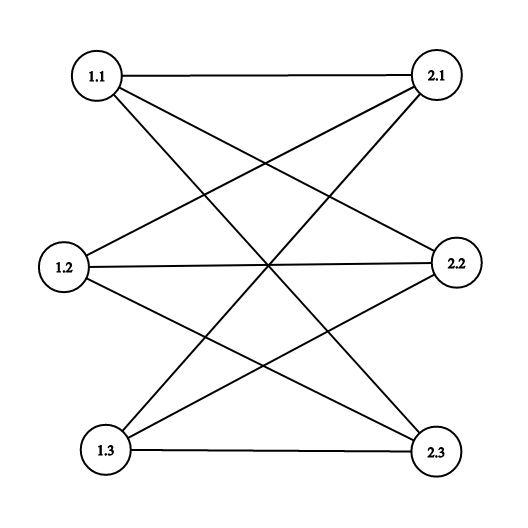
\includegraphics[scale=.3]{images/graph.png}
		\end{center}
	\caption{Grafo de traslado sin costes}\label{fig:ejer_4_graph}
	\end{center}
\end{figure}


%-----------------------------------------------------------------------------------
		\subsubsection{Solución}\label{subsubsec:sol_ejer_4}
%-----------------------------------------------------------------------------------


\textbf{Variables}

\begin{itemize}

\item $D_{i, j, l}$ : Desgaste causado al camino por el transporte del recurso $i$ partiendo del lugar $1 + j/10$ hasta el lugar $2 + l/10$.

\item $T_{i}$ : Total necesario del recurso $i$.

\item $M_{j, l}$ : Cantidad de recursos m\'inima que debe pasar por el camino partiendo del lugar $1+ j/10$ hasta el lugar $2+l/10$. (Dato del inciso b solamente)

\end{itemize}

\textbf{Variables de decisi\'on:}

\begin{itemize}
\item $X_{i,j,l}$ : Cantidad del recurso $i$ a ser transportado partiendo del lugar $1 + j /10$ hasta el lugar $2 + l /10$.
\end{itemize}

\textbf{Funci\'on objetivo:}

Se desea hallar la mejor distribuci\'on de env\'io de los recursos por los distintos caminos de forma tal que el desgaste de los caminos sea lo menor posible.

$$
\min \sum^{4}_{i=1} \sum^{3}_{j=1} \sum^{3}_{l=1} X_{i, j, l} D_{i, j, l}
$$

\textbf{Restricciones:}

Se necesita que los recursos enviados de cada tipo satisfagan la cantidad necesaria.

$$
\sum^{3}_{j=1} \sum^{3}_{l=1} X_{i, j, l} \geq T_{i} \enspace \forall i
$$

Se necesita tambi\'en que por cada camino pasen al menos 3500 unidades de cualquier recurso para mitigar el desgaste de los caminos. (Parte del inciso b solamente)

$$
\sum^{4}_{i=1} X_{i, j, l} \geq M_{j, l} \enspace \forall j, l
$$

%-----------------------------------------------------------------------------------
	\subsection{Casa Stark}\label{subsec:ejer_5}
%-----------------------------------------------------------------------------------
(Este ejercicio tiene una duración de $15$ minutos.)\\

Ya se encuentran todos los recursos en Winterfell, listos para la batalla, el frío y la oscuridad cubren todo. Los exploradores regresan de su misión informando que los caminantes blancos atacarán en 12 oleadas y calculan el estimado de fuerza de cada una de ellas:

\begin{figure}[h!]%
	\begin{center}
		\begin{tabular}{|c|c|c|c|c|c|c|} \hline
		Oleada	& 1		& 2		& 3	    & 4		& 5		& 6		\\ \hline
		Fuerza	& 2000	& 3000	& 4000	& 6000	& 8000	& 10000	\\ \hline
		\end{tabular}
		
		\begin{tabular}{|c|c|c|c|c|c|c|} \hline
		Oleada	& 7		& 8		& 9	    & 10	& 11	& 12	\\ \hline
		Fuerza	& 10000	& 6000	& 4000	& 3000	& 2000	& 2000	\\ \hline
		\end{tabular}
	\caption{Fuerza de oleadas}\label{fig:ejer_5_1}
	\end{center}
\end{figure}

Se sabe que cada soldado puede derrotar a un caminante blanco antes de perecer, además se tiene un lugar inicialmente vacío en las cercanías del campo de batalla, ahí las tropas pueden actuar como una fuerza de acción rápida además den descansar y reparar sus armas para continuar luchando, aunque por desgracia este lugar tiene un máximo de 5000 hombres. Las tropas se van enviando constantemente en cada oleada para reforzar la ofensiva. Debido al proceso de movilización, aumentar la cantidad de hombres que se envían a la batalla en cada oleada tiene un costo de 1 por hombre y disminuirlo de 0.5.

\renewcommand{\theenumi}{\alph{enumi}} % enumerate con incisos
% \renewcommand{\theenumi}{\arabic{enumi}} % enumerate con números

\begin{enumerate}

	\item Realice un plan de lucha que permita ganar la batalla con el mínimo de costo posible.
	\item Para que Arya pueda dar el golpe final se tiene que tener en la última oleada una diferencia de poder ganadora para los caminantes 
	blancos de 1000, para que el jefe se confíe y salga al campo de batalla. Teniendo esto en cuenta, ¿qué cambios le harías a la estrategia?

\end{enumerate}

%-----------------------------------------------------------------------------------
		\subsubsection{Sobre el ejercicio}\label{subsubsec:sobre_ejer_5}
%-----------------------------------------------------------------------------------

Este ejercicio está basado en el problema de almacén, en el cual se tiene una producción, una demanda y un almacén. Variar la producción en un periodo de tiempo tiene un costo asociado y se quiere disminuir al mínimo el costo apoyándose en que el almacén puede aportar a la demanda y aceptar el sobrante de la producción. En este ejercicio se muestra que las variables de decisión no siempre están explícitas en el ejercicio, si no que se tienen que crear a partir de la interacción de los datos, ya que las variables de decisión en este caso se definen como:

$$
x_k = x_1 + \sum_{i=1}^{k-1}z_i
$$

donde $z_i$ es la variación de envío de hombres de la i-ésima oleada con respecto a la anterior.

También introduce la idea de utilizar no solo funciones lineales en problemas, si no también no lineales, como el módulo en este caso que se usa en la función objetivo.

$$
f(x) = \sum_{i=2}^{12} 0.75 |z_i| + 0.25 z_i
$$

%-----------------------------------------------------------------------------------
		\subsubsection{Solución}\label{subsubsec:sol_ejer_5}
%-----------------------------------------------------------------------------------

\textbf{Variables de decisión:}

\begin{itemize}
	\item $h_i$: Cantidad de soldados enviados en la oleada i.
\end{itemize}

Sea $z_i$ la diferencia de hombres entre la oleada $i+1$ y la oleada $i$

\begin{itemize}

	\item $h_{i+1} = h_i + z_i$
	\item $h_{i} = h_0 + \sum_{k=1}^{k-1} z_k$
	
\end{itemize}

\textbf{Restricciones:}

Se quiere que en cada oleada la cantidad de soldados sea mayor que la cantidad de caminantes blancos:

$$
\sum_{i=1}^{k} x_i = k h_0 + \sum_{i=1}^{k-1}(k-i)z_i \ge \sum_{i=1}^k d_i \qquad \forall k \in [1,...,12]
$$

Pero en cada oleada no pueden haber más de 5000 soldados superando a los caminantes blancos:

$$
k h_0 + \sum_{i=1}^{k-1}(k-i)z_i - \sum_{i=1}^k d_i \le 5000 \qquad \forall k \in [1,...,12]
$$

La cantidad de soldados enviados por oleadas tiene que ser no negativa:

$$
h_i \ge 0 \qquad \forall i \in [1,...,12]
$$

La restricción de la oleada final viene dado por la restricción siguiente, la cual representa la cantidad total de caminantes blancos hasta la oleada 12 restado con la cantidad total de soldados hasta la oleada 11:

$$
\sum_{i=1}^{12} d_i - 11 h_0 + \sum_{i=1}^{10}(10-i)z_i \ge 1000
$$

\textbf{Función objetivo:}

Se quiere minimizar el cambio entre oleadas, el cambio está expresado en $z_i$, esta variable puede ser negativa o positiva, y por cada valor
positivo se necesita contar 1 y por cada valor negativo se necesita aumentar en 0.5, lo cual se logra mediante la función módulo.

$$
\min \sum_{i=2}^{12} 0.75 |z_i| + 0.25 z_i
$$

\textbf{Detalles:}

El problema no es lineal, debido a que contiene la función módulo. Se deja de tarea a los estdiantes cómo linealizar el problema.\\

Pasos para linealización:

\renewcommand{\theenumi}{\arabic{enumi}} % enumerate con números
\begin{enumerate}
	\item Crear variables $x_1, x_2$ por cada expresión dentro del módulo tal que $x_1 \ge 0$ y $x_2 \le 0$.
	\item Sustituir en el problema la variable por: $x = x_1 + x_2$
	\item Sustituir en el problema las expresiones con módulo con: $|x| = x_1 - x_2$
\end{enumerate}

De esta manera se linealiza el problema, ya que se puede demostrar que $x_1 = 0 \iff x_2 \neq 0$ si $x \neq 0$ lo que indica que ambas variables se comportan como la parte positiva y negativa respectivamente.

%===================================================================================
% Conclusiones
%-----------------------------------------------------------------------------------
\section{Conclusiones} \label{sec:conc}
%-----------------------------------------------------------------------------------

(Este segmento tiene una duración de $10$ minutos.)\\
 
%Se resumirán los resultados más destacados ejercitados en la actividad.
%
%Se puede hacer mención de aplicaciones del método estudiado, posibles investigaciones o repercusiones en la cotidianidad.

Como conclusión se darán los resultados del equipo ganador, basándonos en cuál fue el equipo que dió los valores más acertados y se dará conclusión al juego.\\

Luego se les explicará a los alumnos que en próximas clases se les dará el contenido necesario para que siempre ganen este tipo de juegos, si está bien modelado el problema, recalcando la importancia de este proceso en la resolución de problemas de optimización.

%===================================================================================
% Ejercicios Propuestos
%-----------------------------------------------------------------------------------
\section{Estudio independiente} \label{independ}
%-----------------------------------------------------------------------------------
(Este segmento tiene una duración de $5$ minutos.)\\
 
%Orientar y comentar los ejercicios propuestos que se deseen.
%
%\begin{ejer}
%	De creerlo conveniente puede asignarse tareas para el estudio independiente, o actividades de carácter evaluativo. 
%\end{ejer}
%
%\begin{ejer}
%	 La cantidad de activiades será a conveniencia aunque podría ser de ayuda su justificar de manera coherente el volumen de trabajo.
%\end{ejer}
%
%El esquema de clase es variable y queda sujeto a la voluntad del participante, solo debe ajustarse a los requisitos de la convocatoria oficial.
\begin{ejer}
	Investigar el uso de scipy para resolver problemas de optimización lineal y resolver los 2 primeros problemas con este.
\end{ejer}
El ejercicio anterior tiene como objetivo introducir al estudiante en la representación y solución computacional de ejercicios de optimización lineal a un alto nivel mediante ejercicios sencillos para que no ocupen mucho tiempo de estudio e investigación ya que en próximas clases se darán algoritmos que resuelven este tipo de problemas.

\begin{ejer}
	Investigar cómo se puede eliminar el módulo en un problema de optimización lineal. 
\end{ejer}
El ejercicio anterior dará pie a que los estudiantes investiguen cómo linealizar la función módulo para convertir el problema en uno lineal, lo cual es necesario para introducir los problemas en solucionadores.



%===================================================================================
% Bibliografía
%-----------------------------------------------------------------------------------
\begin{thebibliography}{99}
%-----------------------------------------------------------------------------------
	
	\bibitem{notas} Gemayqzel Bouza Allende. \emph{Optimización Matemática I: Nota de clase}.
		Tema 2: Modelación, 2021.

\end{thebibliography}
%-----------------------------------------------------------------------------------

\label{end}

\end{document}

%===================================================================================